\begin{frame}
\frametitle{Изоляция и группировка ресурсов}
\begin{itemize}
  \item Иногда хочется изолировать одни потоки от других:
  \begin{itemize}
    \item чтобы ошибки в одном потоке не могли повлиять на другие потоки;
    \item наиболее распространненый случай - раздельная память для потоков.
  \end{itemize}
  \item Процесс - контейнер ресурсов ОС:
  \begin{itemize}
    \item процесс группирует вместе ресурсы и потоки, которые работают с этими
    ресурсами (потоков может быть много, но не меньше одного);
    \item потоки внутри одного процесса используют одну и ту же память (таблицу
    страниц);
    \item в идеале процессы независимы друг от друга и не знают друг о друге,
    но по желанию они могут использовать общие участки памяти;
    \item в зрелых ОС существуют другие ресурсы кроме памяти (например, файловые
    дескрипторы).
  \end{itemize}
\end{itemize}
\end{frame}

\begin{frame}
\frametitle{Организация памяти процесса}
\begin{center}
  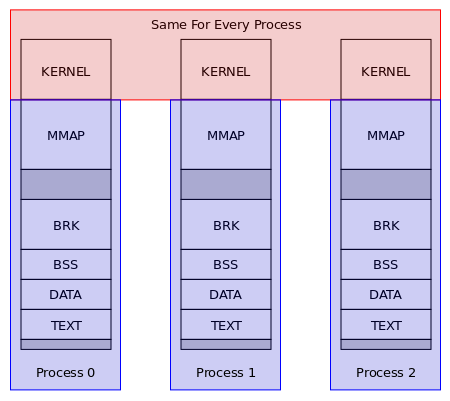
\includegraphics[width=0.45\linewidth]{memmap.png}
\end{center}
\begin{itemize}
  \item Ядро ОС отображается в адресное пространство каждого процесса:
  \begin{itemize}
    \item в таблице страниц каждого процесса есть записи для памяти ядра;
    \item эти записи должны запрещать непривилигерованный доступ к этой памяти.
  \end{itemize}
\end{itemize}
\end{frame}

\begin{frame}
\frametitle{Организация памяти процесса}
\begin{center}
  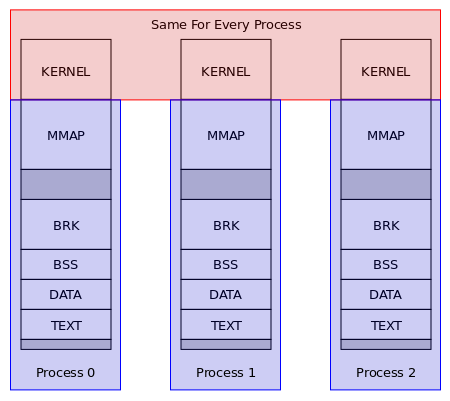
\includegraphics[width=0.45\linewidth]{memmap.png}
\end{center}
\begin{itemize}
  \item Остальная память у каждого процесса своя, но есть но:
  \begin{itemize}
    \item по обоюдному согласию процессы могут иметь общие участки памяти;
    \item память не обязательно физически разделена (хей-хей, page fault).
  \end{itemize}
\end{itemize}
\end{frame}

\begin{frame}
\frametitle{Финальные замечания про процессы}
\begin{itemize}
  \item Процесс - абстракция ОС созданная с использованием аппаратной поддержки:
  \begin{itemize}
    \item в объяснении выше использовалась таблица страниц для организации
    памяти;
    \item мы полагались на прерывания, для переключения потоков внутри процесса
    и между процессами.
  \end{itemize}
  \item Не трудно создать ОС, в которой такой абстракции не будет:
  \begin{itemize}
    \item например, если аппаратной поддержки нет или вам просто не нужна такая
    абстракция;
    \item примеры существуют: MS-DOS;
    \item абстракции не даются бесплатно - вы платите за это
    производительностью.
  \end{itemize}
\end{itemize}
\end{frame}
